%&pdflatex
\documentclass{beamer}

\usepackage{fink}
\usepackage{tikz}
\usepackage{standalone}

\begin{document}

\begin{frame}
  testbeamer \\ %&pdflatex
\documentclass[beamer]{standalone}%

\usepackage{tikz}

\listfiles
\begin{document}%
\begin{standaloneframe}%
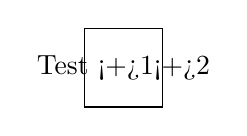
\begin{tikzpicture}
  \draw (0,0) rectangle (1,1) node [midway] {Test \only<+>{1}\only<+>{2}};
\end{tikzpicture}%
\end{standaloneframe}
\end{document}%


\end{frame}

\begin{frame}
  testbeamervrb \\ %&pdflatex
\documentclass[beamer]{standalone}%

\listfiles
\begin{document}
\begin{standaloneframe}[fragile]
  \only<1>{1}
  \only<2>{2}
  \begin{verbatim}
    $Test$%It
  \end{verbatim}
\end{standaloneframe}
\end{document}


\end{frame}

\begin{frame}
  testbeamer1 \\ %&pdflatex
\documentclass[beamer]{standalone}%

\usepackage{tikz}

\listfiles
\begin{document}%
\begin{standaloneframe}<1>%
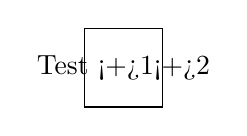
\begin{tikzpicture}
  \draw (0,0) rectangle (1,1) node [midway] {Test \only<+>{1}\only<+>{2}};
\end{tikzpicture}%
\end{standaloneframe}
\end{document}%


\end{frame}

\begin{frame}
  testbeamer2 \\ %&pdflatex
\documentclass[beamer]{standalone}%

\usepackage{tikz}

\listfiles
\begin{document}%
\begin{standaloneframe}<1>[fragile]%
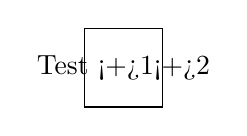
\begin{tikzpicture}
  \draw (0,0) rectangle (1,1) node [midway] {Test \only<+>{1}\only<+>{2}};
\end{tikzpicture}%
\end{standaloneframe}
\end{document}%


\end{frame}

\begin{frame}
  testbeamer3 \\ %&pdflatex
\documentclass[beamer]{standalone}%

\usepackage{tikz}

\listfiles
\begin{document}
\begin{standaloneframe}<1>[<+>][fragile]%
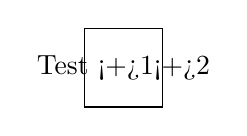
\begin{tikzpicture}
  \draw (0,0) rectangle (1,1) node [midway] {Test \only<+>{1}\only<+>{2}};
\end{tikzpicture}%
\end{standaloneframe}
\end{document}


\end{frame}

\begin{frame}
  testbeamer4 \\ %&pdflatex
\documentclass[beamer]{standalone}%

\usepackage{tikz}

\listfiles
\begin{document}
\begin{standaloneframe}[<+>]%
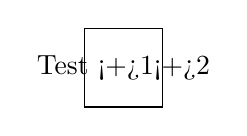
\begin{tikzpicture}
  \draw (0,0) rectangle (1,1) node [midway] {Test \only<+>{1}\only<+>{2}};
\end{tikzpicture}%
\end{standaloneframe}
\end{document}


\end{frame}

\begin{frame}
  testbeamer5 \\ %&pdflatex
\documentclass[beamer]{standalone}%

\usepackage{tikz}

\listfiles
\begin{document}%
\begin{standaloneframe}[<+>][fragile]%
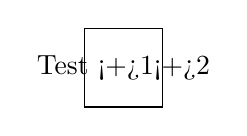
\begin{tikzpicture}
  \draw (0,0) rectangle (1,1) node [midway] {Test \only<+>{1}\only<+>{2}};
\end{tikzpicture}%
\end{standaloneframe}
\end{document}%


\end{frame}

\begin{frame}
  testbeamer1b \\ %&pdflatex
\documentclass[beamer]{standalone}%

\usepackage{tikz}

\listfiles
\begin{document}
\begin{standaloneframe}<*>{Title}{Subtitle}%
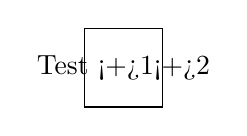
\begin{tikzpicture}
  \draw (0,0) rectangle (1,1) node [midway] {Test \only<+>{1}\only<+>{2}};
\end{tikzpicture}%
\end{standaloneframe}
\end{document}


\end{frame}

\begin{frame}
  testbeamer2b \\ %&pdflatex
\documentclass[beamer]{standalone}%

\usepackage{tikz}

\listfiles
\begin{document}%
\begin{standaloneframe}<*>[label=test]{Title}{Subtitle}%
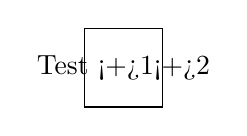
\begin{tikzpicture}
  \draw (0,0) rectangle (1,1) node [midway] {Test \only<+>{1}\only<+>{2}};
\end{tikzpicture}%
\end{standaloneframe}
\end{document}%


\end{frame}

\begin{frame}
  testbeamer3b \\ %&pdflatex
\documentclass[beamer]{standalone}%

\usepackage{tikz}

\listfiles
\begin{document}%
\begin{standaloneframe}<*>[<+>][fragile]{Title}{Subtitle}%
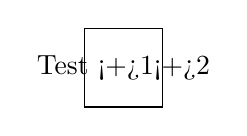
\begin{tikzpicture}
  \draw (0,0) rectangle (1,1) node [midway] {Test \only<+>{1}\only<+>{2}};
\end{tikzpicture}%
\end{standaloneframe}
\end{document}%


\end{frame}

\begin{frame}
  testbeamer4b \\ %&pdflatex
\documentclass[beamer]{standalone}%

\usepackage{tikz}

\listfiles
\begin{document}%
\begin{standaloneframe}[<+>]{Title}{Subtitle}%
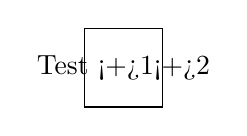
\begin{tikzpicture}
  \draw (0,0) rectangle (1,1) node [midway] {Test \only<+>{1}\only<+>{2}};
\end{tikzpicture}%
\end{standaloneframe}
\end{document}%


\end{frame}

\begin{frame}
  testbeamer5b \\ %&pdflatex
\documentclass[beamer]{standalone}%

\usepackage{tikz}

\listfiles
\begin{document}
\begin{standaloneframe}[<+>][label=test]{Title}{Subtitle}%
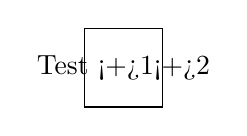
\begin{tikzpicture}
  \draw (0,0) rectangle (1,1) node [midway] {Test \only<+>{1}\only<+>{2}};
\end{tikzpicture}%
\end{standaloneframe}
\end{document}


\end{frame}

\begin{frame}
  testbeamer1c \\ %&pdflatex
\documentclass[beamer]{standalone}%

\usepackage{tikz}

\listfiles
\begin{document}%
\begin{standaloneframe}<*>{Title}
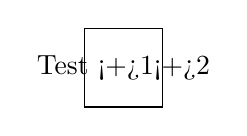
\begin{tikzpicture}
  \draw (0,0) rectangle (1,1) node [midway] {Test \only<+>{1}\only<+>{2}};
\end{tikzpicture}%
\end{standaloneframe}
\end{document}%


\end{frame}

\begin{frame}
  testbeamer2c \\ %&pdflatex
\documentclass[beamer]{standalone}%

\usepackage{tikz}

\listfiles
\begin{document}
\begin{standaloneframe}<*>[label=test]{Title}
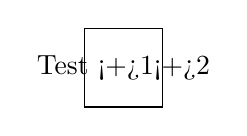
\begin{tikzpicture}
  \draw (0,0) rectangle (1,1) node [midway] {Test \only<+>{1}\only<+>{2}};
\end{tikzpicture}%
\end{standaloneframe}
\end{document}


\end{frame}

\begin{frame}
  testbeamer3c \\ %&pdflatex
\documentclass[beamer]{standalone}%

\usepackage{tikz}

\listfiles
\begin{document}%
\begin{standaloneframe}<*>[<+>][fragile]{Title}
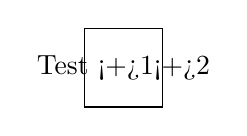
\begin{tikzpicture}
  \draw (0,0) rectangle (1,1) node [midway] {Test \only<+>{1}\only<+>{2}};
\end{tikzpicture}%
\end{standaloneframe}
\end{document}%


\end{frame}

\begin{frame}
  testbeamer4c \\ %&pdflatex
\documentclass[beamer]{standalone}%

\usepackage{tikz}

\listfiles
\begin{document}%
\begin{standaloneframe}[<+>]{Title}
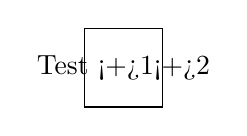
\begin{tikzpicture}
  \draw (0,0) rectangle (1,1) node [midway] {Test \only<+>{1}\only<+>{2}};
\end{tikzpicture}%
\end{standaloneframe}
\end{document}%


\end{frame}

\begin{frame}
  testbeamer5c \\ %&pdflatex
\documentclass[beamer]{standalone}%

\usepackage{tikz}

\listfiles
\begin{document}
\begin{standaloneframe}[<+>][label=test]{Title}
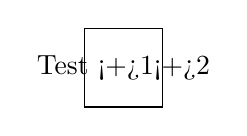
\begin{tikzpicture}
  \draw (0,0) rectangle (1,1) node [midway] {Test \only<+>{1}\only<+>{2}};
\end{tikzpicture}%
\end{standaloneframe}
\end{document}


\end{frame}

\end{document}

